\section{内核的IO模型}

在之前的内核代码当中,基本没有考虑任何的并发和并行的情况,因此,如果是针对
一个 设备同时进行操作,就会导致内核出现崩溃。而常用的解决方式,就是进行加锁。
在内核当中,主要有4种I/O模型,可以实现对设备的访问控制:
\begin{itemize}
  \item 阻塞I/O:最常用,最简单
  \item 非阻塞I/O:可以防止进程阻塞在I/O操作当中
  \item I/O多路复用:允许同时对多个I/O进行控制,通常需要实现poll函数
  \item 信号驱动I/O:异步通信模型
\end{itemize}

\subsection{阻塞/非阻塞式I/O}
常用的阻塞式IO通常采用信号量或者互斥量进行,通过对资源的加锁,解决了并发访问
资源的问题。信号量的加锁方式大致如下:
\begin{code-block}{c}
#include <linux/version.h>
#include <linux/cdev.h>
#include <linux/fs.h>
#include <linux/init.h>
#include <linux/kernel.h>
#include <linux/module.h>
#include <linux/slab.h>
#include <linux/uaccess.h>

#if LINUX_VERSION_CODE < KERNEL_VERSION(5, 0, 0)
#include <linux/device.h>
#endif

#define DEV_NAME "awcloud"
#define BUFFER_LEN 4096
#define MEM_CLEAR 0x1

struct awcloud_sem {
        dev_t             dev_id;
        unsigned int      major;
        unsigned int      minor;
        unsigned int      used_len;
        struct device     *device;
        struct class      *class;
        struct cdev       *cdev;
        char              buffer[BUFFER_LEN];
        // 定义一个信号量
        struct semaphore  sem;
};

static struct awcloud_sem *dev;
static unsigned int major;
module_param(major, uint, 0444);

static int open_awcloud_sem(struct inode *inodep, struct file *filp)
{
        filp->private_data = dev;
        return 0;
}

static int release_awcloud_sem(struct inode *inodep, struct file *filp)
{
        return 0;
}

static ssize_t read_awcloud_sem(struct file *filp,
        char __user *user_buffer, size_t count, loff_t *ppos)
{
        int ret = 0;
        struct awcloud_sem *dev = (struct awcloud_sem *)filp->private_data;

        if (*ppos >= BUFFER_LEN) {
                return count ? -ENXIO:0;
        }

        if (count > (BUFFER_LEN - *ppos)) {
                count = BUFFER_LEN - *ppos;
        }

        // 获取信号量,如果失败,则表示有进程已经在访问了,当前不允许访问
        if (down_interruptible(&dev->sem)) {
                return -ERESTARTSYS;
        }

        // 临界区资源
        if (copy_to_user(user_buffer, (void *)(dev->buffer + *ppos), count)) {
                return -EFAULT;
        }

        *ppos += count;
        ret = count;

        // 释放信号量
        up(&dev->sem);

        return ret;
}

static ssize_t write_awcloud_sem(struct file *filp,
        const char __user *user_buffer, size_t count, loff_t *ppos)
{
        int ret = 0;
        struct awcloud_sem *dev = (struct awcloud_sem *)filp->private_data;

        if (*ppos >= BUFFER_LEN) {
                return count ? -ENXIO:0;
        }

        if (count > BUFFER_LEN - *ppos) {
                count = BUFFER_LEN - *ppos;
        }

        pr_info(
#if defined(__arm__)
                "Calling the write function with count %d, and ppos %lld\n",
#else
                "Calling the write function with count %ld, and ppos %lld\n",
#endif
                count, *ppos);

        if (down_interruptible(&dev->sem)) {
                return -ERESTARTSYS;
        }

        if (copy_from_user(dev->buffer + *ppos, user_buffer, count)) {
                ret = -EFAULT;
                return ret;
        }

        *ppos += count;
        if (*ppos > dev->used_len) {
                dev->used_len = *ppos;
        }
        ret = count;

        up(&dev->sem);
        pr_info(
#if defined(__arm__)
                "Release the semaphore of write for count %d\n",
#else
                "Release the semaphore of write for count %ld\n",
#endif
                count);

        return ret;
}

#if LINUX_VERSION_CODE < KERNEL_VERSION(2, 6, 36)
int ioctl_awcloud_sem(struct inode *inodep,
        struct file *filp, unsigned int cmd, unsigned long arg)
{
#else
static long ioctl_awcloud_sem(struct file *filp,
        unsigned int cmd, unsigned long arg)
{
        //struct inode *inodep = file_inode(filp);
#endif
        struct awcloud_sem *dev = (struct awcloud_sem *)filp->private_data;

        switch (cmd) {
        case MEM_CLEAR:
                if (down_interruptible(&dev->sem)) {
                        return -ERESTARTSYS;
                }

                memset(dev->buffer, 0, BUFFER_LEN);
                dev->used_len = 0;

                up(&dev->sem);

                pr_info("Set Kernel Buffer to Zero\n");
                break;
        default:
                return -EINVAL;
        }
        return 0;
}

static loff_t llseek_awcloud_sem(struct file *filp,
        loff_t offset, int whence)
{
        loff_t ret = 0;
        struct awcloud_sem *dev = (struct awcloud_sem *)filp->private_data;

        pr_info(
                "Calling the llseek function of this device,"
                "and offset is %lld , whence is %d\n", offset, whence);
        switch (whence) {
        case SEEK_SET:
                if (offset < 0) {
                        ret = -EINVAL;
                        break;
                }
                if ((unsigned int)offset > BUFFER_LEN) {
                        ret = -EINVAL;
                        break;
                }
                filp->f_pos = (unsigned int) offset;
                ret = filp->f_pos;
                break;
        case SEEK_CUR:
                if ((filp->f_pos + offset) > BUFFER_LEN) {
                        ret = -EINVAL;
                        break;
                }
                if ((filp->f_pos + offset) < 0) {
                        ret = -EINVAL;
                        break;
                }
                filp->f_pos += offset;
                ret = filp->f_pos;
                break;
        case SEEK_END:
                if ((filp->f_pos + offset) > BUFFER_LEN) {
                        ret = -EINVAL;
                        break;
                }
                if ((filp->f_pos + offset) < 0) {
                        ret = -EINVAL;
                        break;
                }
                if ((dev->used_len+offset) > BUFFER_LEN) {
                        ret = -EINVAL;
                        break;
                }
                filp->f_pos = dev->used_len + offset;
                ret = filp->f_pos;
                break;
        default:
                ret = -EINVAL;
                break;
        }

        return ret;
}

static const struct file_operations awcloud_sem_fops = {
        .owner   = THIS_MODULE,
        .open    = open_awcloud_sem,
        .release = release_awcloud_sem,
        .read    = read_awcloud_sem,
        .write   = write_awcloud_sem,
        .llseek  = llseek_awcloud_sem,
#if LINUX_VERSION_CODE < KERNEL_VERSION(2, 6, 0)
        .ioctl   = ioctl_awcloud_sem,
#else
        .compat_ioctl = ioctl_awcloud_sem,
        .unlocked_ioctl = ioctl_awcloud_sem,
#endif
};

static int awcloud_sem_setup_chrdev(struct awcloud_sem *dev)
{
        int result = 0;

        if (major > 0) {
                dev->dev_id = MKDEV(major, 0);
                result = register_chrdev_region(dev->dev_id, 1, DEV_NAME);
        } else {
                result = alloc_chrdev_region(&(dev->dev_id), 0, 1, DEV_NAME);
        }
        if (result) {
                pr_err("Failed to register the char device\n");
                result = -EFAULT;
                goto chrdev_region_err;
        }

        dev->major = MAJOR(dev->dev_id);
        dev->minor = MINOR(dev->dev_id);

        dev->cdev = cdev_alloc();
        if (!dev->cdev) {
                pr_err("Failed to alloc cdev struct\n");
                result = -EFAULT;
                goto cdev_alloc_err;
        }

        dev->cdev->owner = THIS_MODULE;

        cdev_init(dev->cdev, &awcloud_sem_fops);

        result = cdev_add(dev->cdev, dev->dev_id, 1);
        if (result) {
                pr_err("Failed to add awcloud_sem into Linux system\n");
                result = -EFAULT;
                goto cdev_add_err;
        }

        dev->class = class_create(THIS_MODULE, DEV_NAME);
        if (IS_ERR(dev->class)) {
                result = PTR_ERR(dev->class);
                goto class_create_err;
        }

        dev->device = device_create(dev->class, NULL,
                dev->dev_id, NULL, DEV_NAME);
        if (IS_ERR(dev->device)) {
                result = PTR_ERR(dev->device);
                goto device_create_err;
        }

        memset(dev->buffer, 0, BUFFER_LEN);
        dev->used_len = 0;
#if LINUX_VERSION_CODE > KERNEL_VERSION(2, 6, 36) && !defined(init_MUTEX)
        // 初始化信号量
        sema_init(&(dev->sem), 1);
#else
        init_MUTEX(&(dev->sem));
#endif
        return 0;

device_create_err:
        class_destroy(dev->class);
class_create_err:
        cdev_del(dev->cdev);
cdev_alloc_err:
cdev_add_err:
        unregister_chrdev_region(dev->dev_id, 1);
chrdev_region_err:
        return result;
}

static int __init awcloud_sem_init(void)
{
        int result = 0;

        dev = kzalloc(sizeof(struct awcloud_sem), GFP_KERNEL);
        if (!dev) {
                result = -ENOMEM;
                goto finally;
        }
        result = awcloud_sem_setup_chrdev(dev);
        if (0 > result) {
                kfree(dev);
                goto finally;
        }

finally:
        return result;
}

static void __exit awcloud_sem_exit(void)
{
        device_destroy(dev->class, dev->dev_id);
        class_destroy(dev->class);
        cdev_del(dev->cdev);
        unregister_chrdev_region(dev->dev_id, 1);
        kfree(dev);
}

module_init(awcloud_sem_init);
module_exit(awcloud_sem_exit);

MODULE_LICENSE("GPL");
MODULE_AUTHOR("zhangjl@awcloud.com");
\end{code-block}

而互斥量的使用基本和信号量的相同只是需要将代码略微的修改,改动如下:
\begin{code-block}{c}
struct awcloud_mutex {
        dev_t             dev_id;
        unsigned int      major;
        unsigned int      minor;
        unsigned int      used_len;
        struct device     *device;
        struct class      *class;
        struct cdev       *cdev;
        char              buffer[BUFFER_LEN];
        // 定义一个互斥量
        struct mutex      mutex;
};

static long ioctl_awcloud_mutex(struct file *filp,
        unsigned int cmd, unsigned long arg)
{
        ...
        // 获取互斥量
        if (mutex_lock_interruptible(&dev->mutex)) {
                return -ERESTARTSYS;
        }

        ...
        // 释放互斥量
        mutex_unlock(&dev->mutex);
        ...
}

static int awcloud_mutex_setup_chrdev(struct awcloud_mutex *dev)
{
        ...
        // 初始化互斥量
        mutex_init(&dev->mutex);
        ...
}
\end{code-block}

除了使用信号量与互斥量实现阻塞式IO之外,在实际的工程应用当中,一个驱动模块
通常是可以同时支持阻塞式与非阻塞式IO访问的。而先进先出队列(FIFO)就是一种
典型的在考虑内存的互斥保护时需要同时考虑2种不同阻塞模式的类型。

先进先出队列当中,如果为空,则需要将读操作调度出去,但是写的操作可以被唤醒;
当写入数据之后,读操作可以被唤醒,也就是说,如果FIFO为空,则读操作会一直等待
(阻塞),或者调度其他进程进行执行(非阻塞);而如果FIFO为满,则写操作会一直
等待(阻塞),或者调度其他进程(非阻塞)。FIFO的实现,通常需要使用等待队列,
以及信号量/互斥量等进行实现。一个比较完整的支持阻塞/非阻塞的FIFO的示例如下:
\begin{code-block}{c}
#include <linux/version.h>
#include <linux/cdev.h>
#include <linux/fs.h>
#include <linux/init.h>
#include <linux/kernel.h>
#include <linux/module.h>
#include <linux/slab.h>
#include <linux/uaccess.h>
#include <linux/poll.h>

#if LINUX_VERSION_CODE < KERNEL_VERSION(5, 0, 0)
#include <linux/device.h>
#else
#include <linux/sched/signal.h>
#endif

#define DEV_NAME "awcloud"
#define BUFFER_LEN 4096
#define MEM_CLEAR 0x1

struct awcloud_fifo {
        dev_t             dev_id;
        unsigned int      major;
        unsigned int      minor;
        unsigned int      used_len;
        struct device     *device;
        struct class      *class;
        struct cdev       *cdev;
        char              buffer[BUFFER_LEN];
        struct semaphore  sem;
        // 定义读等待队列
        wait_queue_head_t r_wait;
        // 定义写等待队列
        wait_queue_head_t w_wait;
};

static struct awcloud_fifo *dev;
static unsigned int major;
module_param(major, uint, 0444);

static int open_awcloud_fifo(struct inode *inodep, struct file *filp)
{
        filp->private_data = dev;
        return 0;
}

static int release_awcloud_fifo(struct inode *inodep, struct file *filp)
{
        return 0;
}

static ssize_t read_awcloud_fifo(struct file *filp,
        char __user *user_buffer, size_t count, loff_t *ppos)
{
        int ret = 0;
        struct awcloud_fifo *dev = (struct awcloud_fifo *)filp->private_data;

        // 定义一个等待队列wait
        DECLARE_WAITQUEUE(wait, current);

        // 获取信号量
        down(&dev->sem);
        // 将读添加到等待队列当中
        add_wait_queue(&dev->r_wait, &wait);

        // 如果FIFO的内容为空
        if (0 == dev->used_len) {
                // 如果是非阻塞式的读取,则直接返回
                if (filp->f_flags & O_NONBLOCK) {
                        ret = -EAGAIN;
                        goto again_err;
                }
                // 阻塞式的读取
                // 设置当前状态为可中断的
                __set_current_state(TASK_INTERRUPTIBLE);
                // 释放信号量
                up(&dev->sem);
                // 将进程调度出去,当前进程处于休眠状态,可以被其他操作唤醒
                // 唤醒之后,保持在此处。调度出去之后,不占用cpu。
                schedule();

                // 被其他信号中断,当前进程退出
                if (signal_pending(current)) {
                        ret = -ERESTARTSYS;
                        goto out;
                }

                // 被正常唤醒,重新获取信号
                down(&dev->sem);
        }

        if (count > dev->used_len) {
                count = dev->used_len;
        }

        if (copy_to_user(user_buffer, dev->buffer, count)) {
                ret = -EFAULT;
                goto copy_to_user_err;
        }

        // 似乎没有必要???
        memcpy(dev->buffer, dev->buffer+count, dev->used_len-count);
        // 从FIFO读出数据,需要清空部分长度
        dev->used_len -= count;
#if defined(__arm__)
        pr_info("Read %d bytes, current lenth is %d\n", count, dev->used_len);
#else
        pr_info("Read %ld bytes, current lenth is %d\n", count, dev->used_len);
#endif
        // 唤醒写等待队列
        wake_up_interruptible(&dev->w_wait);
        ret = count;

again_err:
copy_to_user_err:
        // 释放信号量
        up(&dev->sem);

out:
        // 移除读等待队列
        remove_wait_queue(&dev->r_wait, &wait);
        // 设置当前的进程状态
        set_current_state(TASK_RUNNING);

        return ret;
}

static ssize_t write_awcloud_fifo(struct file *filp,
        const char __user *user_buffer, size_t count, loff_t *ppos)
{
        int ret = 0;
        struct awcloud_fifo *dev = (struct awcloud_fifo *)filp->private_data;
        // 定义等待队列
        DECLARE_WAITQUEUE(wait, current);

        pr_info(
#if defined(__arm__)
                "Calling the write function with count %d, and ppos %lld\n",
#else
                "Calling the write function with count %ld, and ppos %lld\n",
#endif
                count, *ppos);

        // 获取信号量
        down(&dev->sem);

        // 将写添加到等待队列当中
        add_wait_queue(&dev->w_wait, &wait);

        // 如果FIFO已经写满
        if (BUFFER_LEN == dev->used_len) {
                // 如果是非阻塞式的写入,则直接返回
                if (filp->f_flags & O_NONBLOCK) {
                        ret = -EAGAIN;
                        goto again_err;
                }
                // 阻塞式的写入,由于已经写满,设置当前进程为可中断的休眠
                __set_current_state(TASK_INTERRUPTIBLE);
                // 释放信号量
                up(&dev->sem);
                // 将自己调度出去,不占cpu
                schedule();

                // 如果当前进程被其他信号中断,则直接返回
                if (signal_pending(current)) {
                        ret = -ERESTARTSYS;
                        goto out;
                }

                // 被wake_up_interruptible唤醒,即正常唤醒,则再次获取信号量
                down(&dev->sem);
        }

        if (count > BUFFER_LEN - dev->used_len) {
                count = BUFFER_LEN - dev->used_len;
        }

        if (copy_from_user(dev->buffer+dev->used_len, user_buffer, count)) {
                ret = -EFAULT;
                goto copy_from_user_err;
        }

        dev->used_len += count;
        // 唤醒读等待队列
        wake_up_interruptible(&dev->r_wait);
        ret = count;

again_err:
copy_from_user_err:
        up(&dev->sem);

out:
        // 移除读等待队列
        remove_wait_queue(&dev->w_wait, &wait);
        // 设置当前进程状态为运行
        set_current_state(TASK_RUNNING);

        return ret;
}

#if LINUX_VERSION_CODE < KERNEL_VERSION(2, 6, 36)
int ioctl_awcloud_fifo(struct inode *inodep,
        struct file *filp, unsigned int cmd, unsigned long arg)
{
#else
static long ioctl_awcloud_fifo(struct file *filp,
        unsigned int cmd, unsigned long arg)
{
        //struct inode *inodep = file_inode(filp);
#endif
        struct awcloud_fifo *dev = (struct awcloud_fifo *)filp->private_data;

        switch (cmd) {
        case MEM_CLEAR:
                if (down_interruptible(&dev->sem)) {
                        return -ERESTARTSYS;
                }

                memset(dev->buffer, 0, BUFFER_LEN);
                dev->used_len = 0;

                up(&dev->sem);

                pr_info("Set Kernel Buffer to Zero\n");
                break;
        default:
                return -EINVAL;
        }
        return 0;
}

static loff_t llseek_awcloud_fifo(struct file *filp,
        loff_t offset, int whence)
{
        loff_t ret = 0;
        struct awcloud_fifo *dev = (struct awcloud_fifo *)filp->private_data;

        pr_info(
                "Calling the llseek function of this device,"
                "and offset is %lld , whence is %d\n", offset, whence);
        switch (whence) {
        case SEEK_SET:
                if (offset < 0) {
                        ret = -EINVAL;
                        break;
                }
                if ((unsigned int)offset > BUFFER_LEN) {
                        ret = -EINVAL;
                        break;
                }
                filp->f_pos = (unsigned int) offset;
                ret = filp->f_pos;
                break;
        case SEEK_CUR:
                if ((filp->f_pos + offset) > BUFFER_LEN) {
                        ret = -EINVAL;
                        break;
                }
                if ((filp->f_pos + offset) < 0) {
                        ret = -EINVAL;
                        break;
                }
                filp->f_pos += offset;
                ret = filp->f_pos;
                break;
        case SEEK_END:
                if ((filp->f_pos + offset) > BUFFER_LEN) {
                        ret = -EINVAL;
                        break;
                }
                if ((filp->f_pos + offset) < 0) {
                        ret = -EINVAL;
                        break;
                }
                if ((dev->used_len+offset) > BUFFER_LEN) {
                        ret = -EINVAL;
                        break;
                }
                filp->f_pos = dev->used_len + offset;
                ret = filp->f_pos;
                break;
        default:
                ret = -EINVAL;
                break;
        }

        return ret;
}

static const struct file_operations awcloud_fifo_fops = {
        .owner          = THIS_MODULE,
        .open           = open_awcloud_fifo,
        .release        = release_awcloud_fifo,
        .read           = read_awcloud_fifo,
        .write          = write_awcloud_fifo,
        .llseek         = llseek_awcloud_fifo,
#if LINUX_VERSION_CODE < KERNEL_VERSION(2, 6, 0)
        .ioctl          = ioctl_awcloud_fifo,
#else
        .compat_ioctl   = ioctl_awcloud_fifo,
        .unlocked_ioctl = ioctl_awcloud_fifo,
#endif
};

static int awcloud_fifo_setup_chrdev(struct awcloud_fifo *dev)
{
        int result = 0;

        if (major > 0) {
                dev->dev_id = MKDEV(major, 0);
                result = register_chrdev_region(dev->dev_id, 1, DEV_NAME);
        } else {
                result = alloc_chrdev_region(&(dev->dev_id), 0, 1, DEV_NAME);
        }
        if (result) {
                pr_err("Failed to register the char device\n");
                result = -EFAULT;
                goto chrdev_region_err;
        }

        dev->major = MAJOR(dev->dev_id);
        dev->minor = MINOR(dev->dev_id);

        dev->cdev = cdev_alloc();
        if (!dev->cdev) {
                pr_err("Failed to alloc cdev struct\n");
                result = -EFAULT;
                goto cdev_alloc_err;
        }

        dev->cdev->owner = THIS_MODULE;

        cdev_init(dev->cdev, &awcloud_fifo_fops);

        result = cdev_add(dev->cdev, dev->dev_id, 1);
        if (result) {
                pr_err("Failed to add awcloud_fifo into Linux system\n");
                result = -EFAULT;
                goto cdev_add_err;
        }

        dev->class = class_create(THIS_MODULE, DEV_NAME);
        if (IS_ERR(dev->class)) {
                result = PTR_ERR(dev->class);
                goto class_create_err;
        }

        dev->device = device_create(dev->class, NULL,
                dev->dev_id, NULL, DEV_NAME);
        if (IS_ERR(dev->device)) {
                result = PTR_ERR(dev->device);
                goto device_create_err;
        }

        memset(dev->buffer, 0, BUFFER_LEN);
        dev->used_len = 0;
#if LINUX_VERSION_CODE > KERNEL_VERSION(2, 6, 36) && !defined(init_MUTEX)
        sema_init(&(dev->sem), 1);
#else
        init_MUTEX(&(dev->sem));
#endif

        // 初始化读等待队列
        init_waitqueue_head(&dev->r_wait);
        // 初始化写等待队列
        init_waitqueue_head(&dev->w_wait);
        return 0;

device_create_err:
        class_destroy(dev->class);
class_create_err:
        cdev_del(dev->cdev);
cdev_alloc_err:
cdev_add_err:
        unregister_chrdev_region(dev->dev_id, 1);
chrdev_region_err:
        return result;
}

static int __init awcloud_fifo_init(void)
{
        int result = 0;

        dev = kzalloc(sizeof(struct awcloud_fifo), GFP_KERNEL);
        if (!dev) {
                result = -ENOMEM;
                goto finally;
        }
        result = awcloud_fifo_setup_chrdev(dev);
        if (0 > result) {
                kfree(dev);
                goto finally;
        }

finally:
        return result;
}

static void __exit awcloud_fifo_exit(void)
{
        device_destroy(dev->class, dev->dev_id);
        class_destroy(dev->class);
        cdev_del(dev->cdev);
        unregister_chrdev_region(dev->dev_id, 1);
        kfree(dev);
}

module_init(awcloud_fifo_init);
module_exit(awcloud_fifo_exit);

MODULE_LICENSE("GPL");
MODULE_AUTHOR("zhangjl@awcloud.com");
\end{code-block}

\subsection{IO多路复用}
实现设备IO的多路复用,需要实现poll函数。需要注意,从4.20版本之后poll函数的
定义存在一些变化,在4.20版本之前,poll函数的定义如下:
\begin{code-block}{c}
unsigned int (*poll) (struct file *, struct poll_table_struct *);
\end{code-block}
而在此之后,poll函数的定义变更为如下的形式:
\begin{code-block}{c}
__poll_t (*poll) (struct file *, struct poll_table_struct *);
\end{code-block}
其中,其中\_\_poll\_t实际上是unsigned int的一个别名,而poll函数的第二个参数,
则表示一个等待队列。在上面的代码基础上,我们可以实现一个设备IO的多路复用功能。
代码的改动如下:
\begin{code-block}{c}
#if LINUX_VERSION_CODE < KERNEL_VERSION(4, 20, 0)
unsigned int poll_awcloud_fifo(
        struct file *filp, struct poll_table_struct *wait)
{
        unsigned int mask = 0;
#else
__poll_t poll_awcloud_fifo(
        struct file *filp, struct poll_table_struct *wait)
{
        __poll_t mask = 0;
#endif
        struct awcloud_fifo *dev = (struct awcloud_fifo *)filp->private_data;

        down(&dev->sem);
        // 添加到可能唤醒IO操作的等待队列当中
        poll_wait(filp, &dev->r_wait, wait);
        poll_wait(filp, &dev->w_wait, wait);

        // 如果FIFO的队列不为空
        if (dev->used_len) {
                // 用户可以进行读取
                mask |= POLLIN | POLLRDNORM;
        }

        // 如果FIFO不满
        if (BUFFER_LEN != dev->used_len) {
                // 用户可以进行写入
                mask |= POLLOUT | POLLWRNORM;
        }
        up(&dev->sem);

        // 用户空间根据mask的值,确定设备是否可读可写
        return mask;
}

static const struct file_operations awcloud_fifo_fops = {
        .owner          = THIS_MODULE,
        .open           = open_awcloud_fifo,
        .release        = release_awcloud_fifo,
        .read           = read_awcloud_fifo,
        .write          = write_awcloud_fifo,
        .llseek         = llseek_awcloud_fifo,
        .poll           = poll_awcloud_fifo,
#if LINUX_VERSION_CODE < KERNEL_VERSION(2, 6, 0)
        .ioctl          = ioctl_awcloud_fifo,
#else
        .compat_ioctl   = ioctl_awcloud_fifo,
        .unlocked_ioctl = ioctl_awcloud_fifo,
#endif
};
\end{code-block}
用户态的多路IO复用通常包括了select,poll和epoll等。以上述的驱动代码为例,我们
可以以select或者epoll的方式对其进行操作,具体参照下列代码:
\begin{code-block}{c}
#include <stdio.h>
#include <fcntl.h>
#include <unistd.h>
#include <sys/ioctl.h>
#if SELECT
#include <sys/select.h>
#elif EPOLL
#include <sys/epoll.h>
#include <strings.h>
#endif

int main(int argc, char *argv[])
{
        int fd;
        int num;

        fd = open("/dev/awcloud0", O_RDWR|O_NONBLOCK);
        if (0 > fd) {
                printf("Cannot open the devices file\n");
                return -1;
        }

#if SELECT
        fd_set read_fds;
        fd_set write_fds;

        while (1) {
                FD_ZERO(&read_fds);
                FD_ZERO(&write_fds);
                FD_SET(fd, &read_fds);
                FD_SET(fd, &write_fds);
                select(fd + 1, &read_fds, &write_fds, NULL, NULL);
                if (FD_ISSET(fd, &read_fds)) {
                        printf("Poll monitor: can be read\n");
                }
                if (FD_ISSET(fd, &write_fds)) {
                        printf("Poll monitor: can be written\n");
                }
        }
#elif EPOLL
        struct epoll_event ev_awcloud;
        int err;
        int epoll_fd;

        epoll_fd = epoll_create(1);
        if (0 > epoll_fd) {
                perror("epoll_create()");
                return -1;
        }
        bzero(&ev_awcloud, sizeof(struct epoll_event));
        ev_awcloud.events = EPOLLIN | EPOLLPRI;
        err = epoll_ctl(epoll_fd, EPOLL_CTL_ADD, fd, &ev_awcloud);
        if (0 > err) {
                perror("epoll_ctl()");
                return -1;
        }

        err = epoll_wait(epoll_fd, &ev_awcloud, 1, 10000);
        if (0 > err) {
                perror("epoll_wait()");
                return -1;
        } else if (0 == err) {
                printf("No data input with in 10 seconds\n");
        } else {
                printf("FIFO is not empty\n");
        }

        err = epoll_ctl(epoll_fd, EPOLL_CTL_DEL, fd, &ev_awcloud);
        if (0 > err) {
                perror("epoll_ctl()");
                return -1;
        }
#elif WRITE
        char content[] = "hello world";
        ssize_t lenth = 0;

        lenth = write(fd, content, sizeof(content)/sizeof(char));
        if (0 > lenth) {
                printf("Cannot write any thing to devices\n");
                close(fd);
                return -1;
        }
#elif READ
        char buffer[1024];
        ssize_t lenth = 0;

        lenth = read(fd, buffer, 1024);
        if (0 > lenth) {
                printf("Cannot read any thing from devices\n");
                close(fd);
                return -1;
        }
        printf("Read the content from device with :%s, %d\n", buffer, lenth);
        lenth = read(fd, buffer, 1024);
        printf("Read the content from device with :%s, %d\n", buffer, lenth);
#elif CLEAR
        if (0 > ioctl(fd, 0x1)) {
                printf("Cannot clean the device content\n");
                close(fd);
                return -1;
        }
#endif
        close(fd);
        return 0;
}
\end{code-block}

\subsection{信号I/O}
信号IO,有时也称之为异步IO。也就是说,每次IO事件发生之后,内核驱动发送
一个信号,通知内核或者用户空间的程序;而对应监听该信号的程序,一旦接收到该
信号,则采取相应的行动。
信号驱动IO,其主要就是需要实现一个异步等待队列,通过这个异步队列,进行信号的
发送。如果在上述代码的基础上,做一些简要的修改,就可以实现该驱动的信号驱动
模式。相应的改动如下:
\begin{code-block}{c}
struct awcloud_async {
        dev_t                dev_id;
        unsigned int         major;
        unsigned int         minor;
        unsigned int         used_len;
        struct device        *device;
        struct class         *class;
        struct cdev          *cdev;
        // 定义一个异步队列
        struct fasync_struct *async_queue;
        char                 buffer[BUFFER_LEN];
        struct semaphore     sem;
        wait_queue_head_t    r_wait;
        wait_queue_head_t    w_wait;
};

static int fasync_awcloud_async(int fd, struct file *filp, int on)
{
        struct awcloud_async *dev = (struct awcloud_async *)filp->private_data;

        // 通过fasync_helper实现异步队列的初始化操作
        return fasync_helper(fd, filp, on, &dev->async_queue);
}

static int release_awcloud_async(struct inode *inodep, struct file *filp)
{
        // 释放异步队列
        fasync_awcloud_async(-1, filp, 0);
        return 0;
}

static ssize_t write_awcloud_async(struct file *filp,
        const char __user *user_buffer, size_t count, loff_t *ppos)
{
        ...
        wake_up_interruptible(&dev->r_wait);
        ret = count;

        // 判断异步队列是否为空
        if (dev->async_queue) {
                // 向异步队列发送SIGIO信号,POLL_IN表示用户空间可以进行读取了
                kill_fasync(&dev->async_queue, SIGIO, POLL_IN);
                pr_debug("%s kill SIGIO", __func__);
        }

again_err:
copy_from_user_err:
        up(&dev->sem);

out:
        remove_wait_queue(&dev->w_wait, &wait);
        set_current_state(TASK_RUNNING);

        return ret;
}

static ssize_t read_awcloud_async(struct file *filp,
        char __user *user_buffer, size_t count, loff_t *ppos)
{
        ...
        wake_up_interruptible(&dev->w_wait);
        if (dev->async_queue) {
                // 向异步队列发送SIGIO信号,POLL_OUT表示用户可以进行写操作了
                kill_fasync(&dev->async_queue, SIGIO, POLL_OUT);
                pr_debug("%s kill SIGIO", __func__);
        }
        ret = count;

again_err:
copy_to_user_err:
        up(&dev->sem);

out:
        remove_wait_queue(&dev->r_wait, &wait);
        set_current_state(TASK_RUNNING);

        return ret;
}

static const struct file_operations awcloud_async_fops = {
        .owner          = THIS_MODULE,
        .open           = open_awcloud_async,
        .release        = release_awcloud_async,
        .read           = read_awcloud_async,
        .write          = write_awcloud_async,
        .llseek         = llseek_awcloud_async,
        .poll           = poll_awcloud_async,
        // 实现异步IO,则必须实现fasync函数
        .fasync         = fasync_awcloud_async,
#if LINUX_VERSION_CODE < KERNEL_VERSION(2, 6, 0)
        .ioctl          = ioctl_awcloud_async,
#else
        .compat_ioctl   = ioctl_awcloud_async,
        .unlocked_ioctl = ioctl_awcloud_async,
#endif
};
\end{code-block}

\section{多设备管理}
很多情况下,Linux系统当中相同的设备总是会有多个,因此,一个驱动模块,驱使
多个相同的设备就成了必然。在之前的描述当中,我们仅仅实现了单个设备的管理,
接下来,我们看看内核当中对多设备的管理实现。需要注意,同类型的设备,在系统当中
的设备名称是不同的,否则会出现错误。下面是完整的代码:
\begin{code-block}{c}
#include <linux/version.h>
#include <linux/cdev.h>
#include <linux/fs.h>
#include <linux/init.h>
#include <linux/kernel.h>
#include <linux/module.h>
#include <linux/slab.h>
#include <linux/uaccess.h>
#include <linux/poll.h>

#if LINUX_VERSION_CODE < KERNEL_VERSION(5, 0, 0)
#include <linux/device.h>
#else
#include <linux/sched/signal.h>
#endif

#define DEV_NAME "awcloud"
#define BUFFER_LEN 4096
#define MEM_CLEAR 0x1

struct awcloud_async {
        unsigned int         used_len;
        struct device        *device;
        struct class         *class;
        struct fasync_struct *async_queue;
        char                 buffer[BUFFER_LEN];
        struct semaphore     sem;
        struct cdev          cdev;
        wait_queue_head_t    r_wait;
        wait_queue_head_t    w_wait;
};

static struct awcloud_async *dev;
static unsigned int major;
static unsigned int num_devices;
module_param(major, uint, 0444);
module_param(num_devices, uint, 0444);

static int open_awcloud_async(struct inode *inodep, struct file *filp)
{
        struct awcloud_async *dev = container_of(
                inodep->i_cdev, struct awcloud_async, cdev);
        filp->private_data = dev;
        return 0;
}

static int release_awcloud_async(struct inode *inodep, struct file *filp)
{
        // 释放异步通知
        fasync_awcloud_async(-1, filp, 0);
        return 0;
}

static ssize_t read_awcloud_async(struct file *filp,
        char __user *user_buffer, size_t count, loff_t *ppos)
{
        int ret = 0;
        struct awcloud_async *dev = (struct awcloud_async *)filp->private_data;

        DECLARE_WAITQUEUE(wait, current);

        down(&dev->sem);
        add_wait_queue(&dev->r_wait, &wait);

        if (0 == dev->used_len) {
                if (filp->f_flags & O_NONBLOCK) {
                        ret = -EAGAIN;
                        goto again_err;
                }
                __set_current_state(TASK_INTERRUPTIBLE);
                up(&dev->sem);
                schedule();

                if (signal_pending(current)) {
                        ret = -ERESTARTSYS;
                        goto out;
                }
                down(&dev->sem);
        }

        if (count > dev->used_len) {
                count = dev->used_len;
        }

        if (copy_to_user(user_buffer, dev->buffer, count)) {
                ret = -EFAULT;
                goto copy_to_user_err;
        }

        //memcpy(dev->buffer, dev->buffer+count, dev->used_len-count);
        dev->used_len -= count;
#if defined(__arm__)
        pr_info("Read %d bytes, current lenth is %d\n", count, dev->used_len);
#else
        pr_info("Read %ld bytes, current lenth is %d\n", count, dev->used_len);
#endif
        wake_up_interruptible(&dev->w_wait);
        if (dev->async_queue) {
                kill_fasync(&dev->async_queue, SIGIO, POLL_OUT);
                pr_debug("%s kill SIGIO", __func__);
        }
        ret = count;

again_err:
copy_to_user_err:
        up(&dev->sem);

out:
        remove_wait_queue(&dev->r_wait, &wait);
        set_current_state(TASK_RUNNING);

        return ret;
}

static ssize_t write_awcloud_async(struct file *filp,
        const char __user *user_buffer, size_t count, loff_t *ppos)
{
        int ret = 0;
        struct awcloud_async *dev = (struct awcloud_async *)filp->private_data;
        DECLARE_WAITQUEUE(wait, current);

        pr_info(
#if defined(__arm__)
                "Calling the write function with count %d, and ppos %lld\n",
#else
                "Calling the write function with count %ld, and ppos %lld\n",
#endif
                count, *ppos);

        down(&dev->sem);
        add_wait_queue(&dev->w_wait, &wait);

        if (BUFFER_LEN == dev->used_len) {
                if (filp->f_flags & O_NONBLOCK) {
                        ret = -EAGAIN;
                        goto again_err;
                }
                __set_current_state(TASK_INTERRUPTIBLE);
                up(&dev->sem);
                schedule();
                if (signal_pending(current)) {
                        ret = -ERESTARTSYS;
                        goto out;
                }
                down(&dev->sem);
        }

        if (count > BUFFER_LEN - dev->used_len) {
                count = BUFFER_LEN - dev->used_len;
        }

        if (copy_from_user(dev->buffer+dev->used_len, user_buffer, count)) {
                ret = -EFAULT;
                goto copy_from_user_err;
        }

        dev->used_len += count;
        wake_up_interruptible(&dev->r_wait);
        ret = count;

        if (dev->async_queue) {
                kill_fasync(&dev->async_queue, SIGIO, POLL_IN);
                pr_debug("%s kill SIGIO", __func__);
        }

again_err:
copy_from_user_err:
        up(&dev->sem);

out:
        remove_wait_queue(&dev->w_wait, &wait);
        set_current_state(TASK_RUNNING);

        return ret;
}

#if LINUX_VERSION_CODE < KERNEL_VERSION(2, 6, 36)
int ioctl_awcloud_async(struct inode *inodep,
        struct file *filp, unsigned int cmd, unsigned long arg)
{
#else
static long ioctl_awcloud_async(struct file *filp,
        unsigned int cmd, unsigned long arg)
{
        //struct inode *inodep = file_inode(filp);
#endif
        struct awcloud_async *dev = (struct awcloud_async *)filp->private_data;

        pr_info("Calling the ioctl function\n");
        switch (cmd) {
        case MEM_CLEAR:
                if (down_interruptible(&dev->sem)) {
                        return -ERESTARTSYS;
                }

                memset(dev->buffer, 0, BUFFER_LEN);
                dev->used_len = 0;

                up(&dev->sem);

                pr_info("Set Kernel Buffer to Zero\n");
                break;
        default:
                return -EINVAL;
        }
        return 0;
}

static loff_t llseek_awcloud_async(struct file *filp,
        loff_t offset, int whence)
{
        loff_t ret = 0;
        struct awcloud_async *dev = (struct awcloud_async *)filp->private_data;

        pr_info(
                "Calling the llseek function of this device,"
                "and offset is %lld , whence is %d\n", offset, whence);
        switch (whence) {
        case SEEK_SET:
                if (offset < 0) {
                        ret = -EINVAL;
                        break;
                }
                if ((unsigned int)offset > BUFFER_LEN) {
                        ret = -EINVAL;
                        break;
                }
                filp->f_pos = (unsigned int) offset;
                ret = filp->f_pos;
                break;
        case SEEK_CUR:
                if ((filp->f_pos + offset) > BUFFER_LEN) {
                        ret = -EINVAL;
                        break;
                }
                if ((filp->f_pos + offset) < 0) {
                        ret = -EINVAL;
                        break;
                }
                filp->f_pos += offset;
                ret = filp->f_pos;
                break;
        case SEEK_END:
                if ((filp->f_pos + offset) > BUFFER_LEN) {
                        ret = -EINVAL;
                        break;
                }
                if ((filp->f_pos + offset) < 0) {
                        ret = -EINVAL;
                        break;
                }
                if ((dev->used_len+offset) > BUFFER_LEN) {
                        ret = -EINVAL;
                        break;
                }
                filp->f_pos = dev->used_len + offset;
                ret = filp->f_pos;
                break;
        default:
                ret = -EINVAL;
                break;
        }

        return ret;
}

#if LINUX_VERSION_CODE < KERNEL_VERSION(4, 20, 0)
unsigned int poll_awcloud_async(
        struct file *filp, struct poll_table_struct *wait)
{
        unsigned int mask = 0;
#else
__poll_t poll_awcloud_async(
        struct file *filp, struct poll_table_struct *wait)
{
        __poll_t mask = 0;
#endif
        struct awcloud_async *dev = (struct awcloud_async *)filp->private_data;

        down(&dev->sem);
        poll_wait(filp, &dev->r_wait, wait);
        poll_wait(filp, &dev->w_wait, wait);
        if (dev->used_len) {
                mask |= POLLIN | POLLRDNORM;
        }
        if (BUFFER_LEN != dev->used_len) {
                mask |= POLLOUT | POLLWRNORM;
        }
        up(&dev->sem);

        return mask;
}

static int fasync_awcloud_async(int fd, struct file *filp, int on)
{
        struct awcloud_async *dev = (struct awcloud_async *)filp->private_data;

        return fasync_helper(fd, filp, on, &dev->async_queue);
}

static int release_awcloud_async(struct inode *inodep, struct file *filp)
{
        // 释放异步通知
        fasync_awcloud_async(-1, filp, 0);
        return 0;
}

const static struct file_operations awcloud_async_fops = {
        .owner          = THIS_MODULE,
        .open           = open_awcloud_async,
        .release        = release_awcloud_async,
        .read           = read_awcloud_async,
        .write          = write_awcloud_async,
        .llseek         = llseek_awcloud_async,
        .poll           = poll_awcloud_async,
        .fasync         = fasync_awcloud_async,
#if LINUX_VERSION_CODE < KERNEL_VERSION(2, 6, 0)
        .ioctl          = ioctl_awcloud_async,
#else
        .compat_ioctl   = ioctl_awcloud_async,
        .unlocked_ioctl = ioctl_awcloud_async,
#endif
};

static int awcloud_async_setup_chrdev(struct awcloud_async *dev, int index)
{
        int result = 0;
        char device_name[10];
        // 不同的设备的设备号不同
        dev_t dev_id = MKDEV(major, index);

        dev->cdev.owner = THIS_MODULE;
        // 每个设备都需要绑定操作函数
        cdev_init(&dev->cdev, &awcloud_async_fops);

        // 每次增加一个设备
        if (cdev_add(&dev->cdev, dev_id, 1)) {
                pr_err("Failed to add char dev into system\n");
                result = -1;
                goto cdev_add_err;
        }

        sprintf(device_name, DEV_NAME"%d", index);
        // 创建设备文件
        dev->device = device_create(
                dev->class, NULL, dev_id, NULL, device_name);
        if (IS_ERR(dev->device)) {
                result = -1;
                goto device_create_err;
        }

        memset(dev->buffer, 0, BUFFER_LEN);
        dev->used_len = 0;

        // 每个设备文件都需要对应各自的信号量
        // 以及等待队列
        sema_init(&(dev->sem), 1);
        init_waitqueue_head(&dev->r_wait);
        init_waitqueue_head(&dev->w_wait);
        return result;

device_create_err:
        cdev_del(&dev->cdev);
cdev_add_err:
        return result;
}

static void release_awcloud_async_chrdev(struct awcloud_async *dev, int index)
{
        dev_t dev_id = MKDEV(major, index);

        device_destroy(dev->class, dev_id);
        cdev_del(&dev->cdev);
}

static int __init awcloud_async_init(void)
{
        int result = 0;
        int index = 0;
        int tmp[3] = {0};
        dev_t dev_id;
        struct class *class = NULL;

        if (0 >= num_devices) {
                num_devices = 1;
        }

        // 根据设备的个数进行对应的内存申请和分配
        dev = kzalloc(sizeof(struct awcloud_async) * num_devices, GFP_KERNEL);
        if (!dev) {
                result = -ENOMEM;
                goto finally;
        }

        if (major > 0) {
                dev_id = MKDEV(major, 0);
                result = register_chrdev_region(
                        dev_id, num_devices, DEV_NAME);
        } else {
                result = alloc_chrdev_region(
                        &dev_id, 0, num_devices, DEV_NAME);
        }

        if (result) {
                pr_err("Failed to alloc the char dev number\n");
                result = -EFAULT;
                goto alloc_dev_id_err;
        }

        // 相同类型的所有设备的主设备号是相同的
        major = MAJOR(dev_id);

        // 相同类型的所有设备的class是相同的,并且需要注意,
        // 无论相同类型的设备有多少,class_create函数总计只能
        // 调用一次,否则会导致内核错误
        class = class_create(THIS_MODULE, DEV_NAME);
        if (IS_ERR(class)) {
                result = -1;
                goto class_create_err;
        }

        // 根据设备的数量,进行内核驱动设备的生成与实现
        for (index = 0; index < num_devices; index++) {
                (dev+index)->class = class;
                tmp[index] = awcloud_async_setup_chrdev(dev+index, index);
                result |= tmp[index];
        }

        // 异常情况处理
        if (result) {
                for (index = 0; index < num_devices; index++) {
                        if (!tmp[index]) {
                                release_awcloud_async_chrdev(dev+index, index);
                        }
                }
                goto setup_chrdev_err;
        }

        return result;

setup_chrdev_err:
        class_destroy(class);
class_create_err:
        unregister_chrdev_region(MKDEV(major, 0), num_devices);
alloc_dev_id_err:
        kfree(dev);
finally:
        return result;
}

static void __exit awcloud_async_exit(void)
{
        int index = 0;

        for (index = 0; index < num_devices; index++) {
                release_awcloud_async_chrdev(dev+index, index);
        }

        class_destroy(dev->class);
        unregister_chrdev_region(MKDEV(major, 0), num_devices);
        kfree(dev);
}

module_init(awcloud_async_init);
module_exit(awcloud_async_exit);

MODULE_LICENSE("GPL");
MODULE_AUTHOR("zhangjl@awcloud.com");
\end{code-block}
代码编译之后,通过指令进行内核模块的加载,指定生成3个对应的设备
\begin{code-block}{bash}
insmod awcloud.ko num_devices=3
\end{code-block}
则会在/dev下生成3个不同的设备文件如下图\nameref{fig:multi_devices}所示:
\begin{figure}[H]
  \centering
  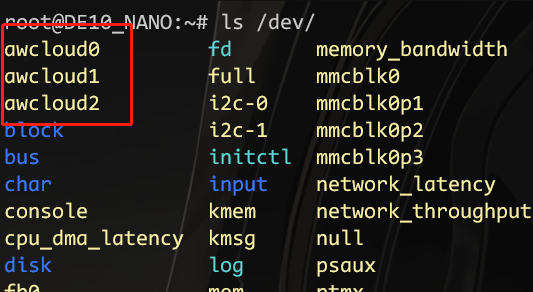
\includegraphics[width=\linewidth]{multi_devices.png}
  \caption{驱动的多设备管理}
  \label{fig:multi_devices}
\end{figure}

\section{Platform驱动模型}
